\section{Overview}

This chapter outlines the methodology employed for image processing and evaluating the quality of the lens. The process involves several steps, from capturing and preprocessing images to analyzing various lens properties. The chapter also describes the architecture of the system, data flow among the system and features a set of scenarios for simple lens evaluation. This chapter concludes with the design of User Interface Design.

\section{Image Acquisition}

\subsection{Camera Setup and Configuration}

\subsection{RAW Image Capture Techniques}

\section{Image Preprocessing}
Images, captured in RAW format using a digital camera, need to be processed before analyzing the lens quality. Image preprocessing ensures that the images are in the optimal condition for subsequent analysis, reducing noise and enhancing feature detection accuracy.

\subsection{Filtering}

Image filtering is a crucial step in image preprocessing; its goal is to enhance the image quality and prepare it for subsequent analysis. Filtering helps in reducing noise, smoothing the image, and highlighting important features.

\textbf{Gaussian blur} is a widely-used smoothing technique that applies a Gaussian function to the image. It effectively reduces noise and detail, providing a smoother and more uniform image. The Gaussian blur is particularly useful in preparing images for feature detection and other analytical processes \cite{gaussian}. 

\subsection{Edge detection}

Edge detection is a crucial step in image processing, used to identify significant transitions in intensity within an image. These transitions often correspond to the boundaries of objects within the scene, making edge detection an essential technique for feature extraction, image segmentation, and object recognition.


\subsection{Feature detection}
Feature detection on the captured image is performed using the \textbf{Scale-Invariant Feature Transform} (SIFT). This algorithm detects and describes local features in images, also referred to as keypoints in the following sections. SIFT is used in computer vision for object recognition, image stitching, and other applications due to its robustness to changes in scale, rotation, and illumination. In this case it is used for analyzing sharpness, PSF, and bokeh \cite{Sift}.

\section{Assessment of lens quality}

The methodology for lens evaluation involves analyzing several properties of the lens, such as sharpness, vignetting, point spread function (PSF), and bokeh. Below are detailed explanations of each part of the evaluation process.

\subsection{Statistical Methods}

Statistical methods used in assessment of lens quality involve the use of mean values and standard deviations to evaluate properties such as sharpness, PSF, and bokeh. For instance, the mean response values of keypoints provide a measure of sharpness, while the standard deviation of pixel values around keypoints gives insights into the bokeh quality. These statistical measures are essential for summarizing the central tendency and variability in the data, allowing for a comprehensive evaluation of the lens's optical performance.

\subsection{Sharpness Analysis}

Sharpness analysis involves calculating the average response value of the detected keypoints. The sharpness is quantified by evaluating the response values (strength) of these keypoints. Higher response values indicate sharper features, which correspond to better lens performance in terms of resolving fine details.

\subsection{Vignetting Analysis}

Vignetting analysis measures the effect of vignetting by comparing the mean intensity values between the center and corners of the grayscale image. Vignetting refers to the reduction of an image's brightness or saturation at the periphery compared to the image center. By dividing the image into specific regions (e.g., center and corners), calculating their mean intensities, and determining the differences, one can quantify the degree of vignetting.

\subsection{Point Spread Function (PSF) Analysis}

The Point Spread Function (PSF) analysis assesses how light from a point source is distributed in the image. This is achieved by summing the pixel values around each detected keypoint and calculating the average of these summed values. The PSF provides insights into the lens's ability to focus light precisely. A narrower PSF indicates better focusing ability, leading to sharper images.

\subsection{Bokeh Analysis}

Bokeh analysis evaluates the aesthetic quality of the out-of-focus areas in an image. This is done by first calculating the standard deviation of pixel values around each keypoint and then averaging these standard deviations. A higher standard deviation indicates a more pronounced bokeh effect, with smoother out-of-focus areas. This analysis helps in understanding how the lens renders out-of-focus highlights and background blur.

\section{System Architecture}

The system architecture of the lens evaluation application is composed of four main components: image acquisition, segmentation and preprocessing, lens property evaluation, and result display. These components work together to capture images from a camera, process and analyze these images, and present the results to the user through a web interface.

\subsection{Image Acquisition Component}
This component interfaces with the camera to capture images in RAW format. It handles camera communication, controls camera settings, and stores the captured images for further processing.

\subsection{Segmentation and Preprocessing Component}
This component processes the captured images to locate and extract calibration elements. Preprocessing may include steps like geometric distortion correction and noise reduction to ensure accurate analysis.

\subsection{Lens Property Evaluation Component}
This is the core analytical component that assesses various lens properties such as sharpness, vignetting, point spread function (PSF), and bokeh. It uses mathematical algorithms to compute metrics and generate scores for each property.

\subsection{Result Display Component}
The results are displayed to the user through a web interface. This component includes functions for visualizing analysis results, managing datasets, and interacting with the application. The design of the user interface is crucial for ensuring usability and accessibility for both advanced users and beginners.

\subsection{System Diagram}

\begin{figure}[h]
\centering

\includegraphics[width=0.99\textwidth]{Images/architecture_diagram.png}
\caption{System Architecture Diagram}
\label{fig:system_architecture}
\end{figure}

\section{Data Flow}

The data flow in the application follows a structured process from image acquisition to result display. Each step is designed to ensure that the captured images are accurately processed and analyzed, and the results are presented in a user-friendly manner.

\subsection{Step-by-Step Data Flow}

\begin{enumerate}
    \item \textbf{Image Acquisition}
    \begin{itemize}
        \item The user sets up the test environment and connects the camera to the application via USB.
        \item The application captures a series of images in RAW format, adjusting settings like aperture and focus distance as needed.
        \item Captured images are stored temporarily for processing.
    \end{itemize}

    \item \textbf{Segmentation and Preprocessing}
    \begin{itemize}
        \item The application locates calibration elements within the captured images using image processing algorithms.
        \item Preprocessing steps, such as geometric distortion correction and minimal noise reduction, are applied to enhance the accuracy of the analysis.
    \end{itemize}

    \item \textbf{Lens Property Evaluation}
    \begin{itemize}
        \item The application evaluates lens properties based on the processed images. This includes analyzing sharpness using the Siemens star, vignetting using images of a white wall, and bokeh using images of a point light source.
        \item Mathematical algorithms compute various metrics, and results are scored and standardized for comparison.
    \end{itemize}

    \item \textbf{Result Display}
    \begin{itemize}
        \item The results are presented to the user through a web interface. Users can view detailed analysis, compare different lenses, and manage datasets.
        \item The interface provides options to save and load session data, enabling repeated analyses and comparisons over time.
    \end{itemize}
\end{enumerate}

\section{Scenarios for Analysis}

To comprehensively evaluate lens properties, the application supports multiple scenarios, each designed to assess different aspects of lens performance.

\subsection{Scenario A: Vignetting Analysis}
\begin{itemize}
    \item \textbf{Setup}: Point the camera at a white wall with even lighting.
    \item \textbf{Procedure}: Capture images at different aperture settings.
    \item \textbf{Analysis}: Evaluate vignetting by measuring the reduction in brightness at the edges compared to the center of the image.
\end{itemize}

\subsection{Scenario B: PSF and Bokeh Analysis}
\begin{itemize}
    \item \textbf{Setup}: Use a point light source, such as a phone flashlight, placed in a dark environment.
    \item \textbf{Procedure}: Capture images at different focus points and aperture settings, ensuring correct exposure.
    \item \textbf{Analysis}: Evaluate the Point Spread Function (PSF) and bokeh characteristics by analyzing the shape and distribution of the defocused light.
\end{itemize}

\subsection{Scenario C: Sharpness and Distortion Analysis}
\begin{itemize}
    \item \textbf{Setup}: Position a printed test chart (including a Siemens star and slanted edges) in front of the camera.
    \item \textbf{Procedure}: Capture images of the test chart.
    \item \textbf{Analysis}: Evaluate sharpness using the Siemens star and slanted edge methods, and assess geometric distortions (barrel and pincushion) by analyzing the grid patterns on the test chart.
\end{itemize}

\subsection{Data Management and Session Handling}
\begin{itemize}
    \item \textbf{Session Protocol}: The application remembers the names and locations of captured files. A dataset consists of multiple scenarios, and each scenario includes a set of photos with different parameters. The parameters used during the capture are also saved with the session data.
    \item \textbf{Dynamic Loading}: Due to the large size of RAW files, the application loads images dynamically as needed for analysis, rather than storing them all in memory.
\end{itemize}

\section{User Interface Design}

The user interface (UI) of the application is designed to be intuitive and user-friendly, catering to both advanced users and beginners. The UI is structured around a main screen for overall navigation and specific screens for various tasks. The following sketches illustrate the key screens and interactions within the application.

\subsection{Main Screen}

The main screen serves as the central hub for the application. It provides options to load and save datasets, inspect the camera status, and run analyses. Users can navigate to different tasks such as capturing images for scenarios, viewing analysis results, and managing session data from this screen.

\begin{figure}[h]
\centering
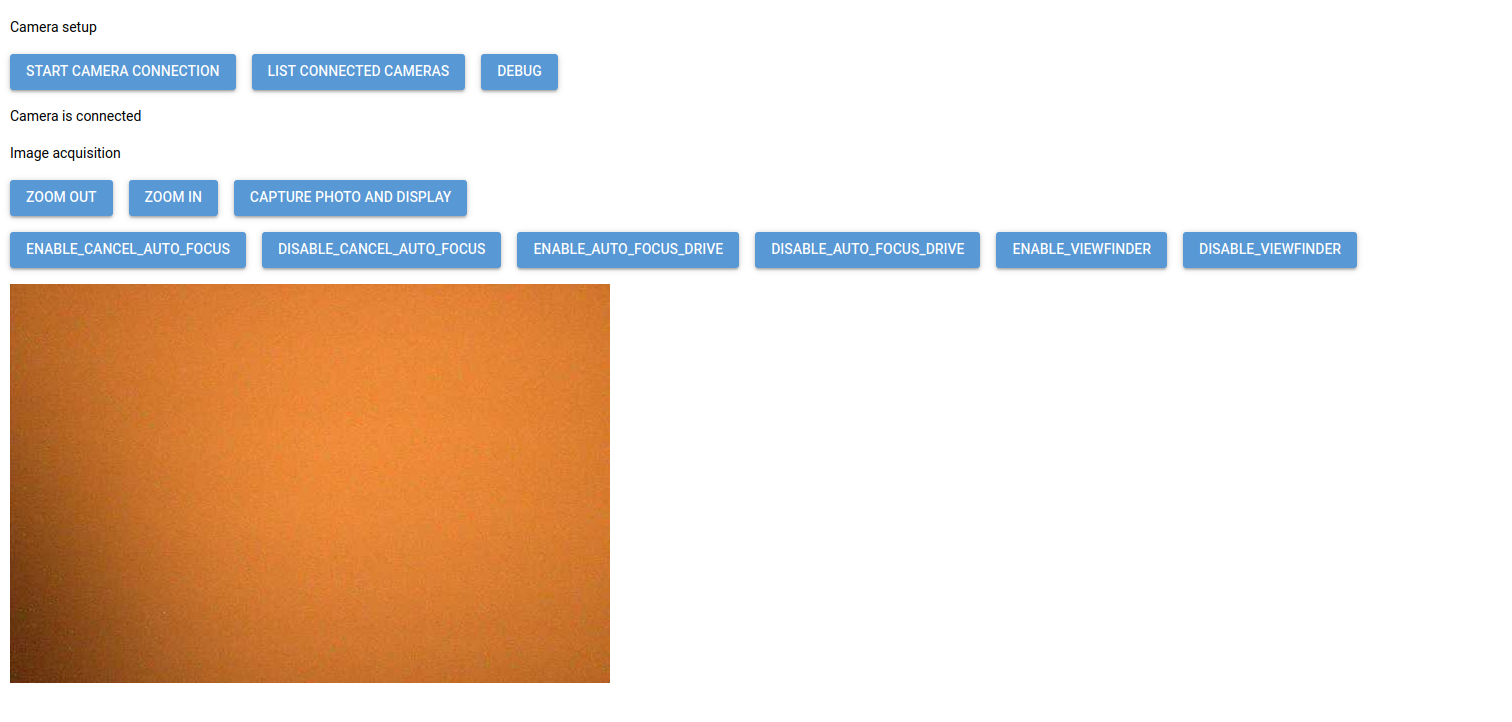
\includegraphics[width=1\textwidth]{Images/ui1.png}
\caption{Main screen with camera connection and photo capture features.}
\label{fig:ui_main_screen}
\end{figure}

\subsection{Scenario Capture Screen}

The scenario capture screen allows users to set up and capture images for different scenarios. Users can adjust camera settings such as aperture and focus distance, and initiate the image capture process. The interface guides the user through the steps required for each scenario, ensuring proper setup and execution.

%% \caption{Sketch of the Scenario Capture Screen}

\subsection{Analysis Results Screen}

The analysis results screen displays the results of the lens property evaluations. Users can view detailed metrics for sharpness, vignetting, PSF, and bokeh, and compare results across different lenses or scenarios.

\begin{figure}[h]
\centering
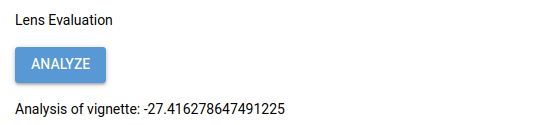
\includegraphics[width=0.8\textwidth]{Images/ui2.png}
\caption{Sketch of the screen with Analyze button and result of vignette analysis.}
\label{fig:ui_main_screen}
\end{figure}

\subsection{Session Management Screen}

The session management screen provides options to save and load session data. Users can manage their datasets, including adding new scenarios and reviewing previously captured images. The interface ensures that all session data is easily accessible and well-organized.

%%\caption{Sketch of the Session Management Screen}
